% Options for packages loaded elsewhere
% Options for packages loaded elsewhere
\PassOptionsToPackage{unicode}{hyperref}
\PassOptionsToPackage{hyphens}{url}
\PassOptionsToPackage{dvipsnames,svgnames,x11names}{xcolor}
%
\documentclass[
  11pt,
  letterpaper,
  DIV=11,
  numbers=noendperiod]{scrartcl}
\usepackage{xcolor}
\usepackage[margin=1in]{geometry}
\usepackage{amsmath,amssymb}
\setcounter{secnumdepth}{5}
\usepackage{iftex}
\ifPDFTeX
  \usepackage[T1]{fontenc}
  \usepackage[utf8]{inputenc}
  \usepackage{textcomp} % provide euro and other symbols
\else % if luatex or xetex
  \usepackage{unicode-math} % this also loads fontspec
  \defaultfontfeatures{Scale=MatchLowercase}
  \defaultfontfeatures[\rmfamily]{Ligatures=TeX,Scale=1}
\fi
\usepackage{lmodern}
\ifPDFTeX\else
  % xetex/luatex font selection
\fi
% Use upquote if available, for straight quotes in verbatim environments
\IfFileExists{upquote.sty}{\usepackage{upquote}}{}
\IfFileExists{microtype.sty}{% use microtype if available
  \usepackage[]{microtype}
  \UseMicrotypeSet[protrusion]{basicmath} % disable protrusion for tt fonts
}{}
\makeatletter
\@ifundefined{KOMAClassName}{% if non-KOMA class
  \IfFileExists{parskip.sty}{%
    \usepackage{parskip}
  }{% else
    \setlength{\parindent}{0pt}
    \setlength{\parskip}{6pt plus 2pt minus 1pt}}
}{% if KOMA class
  \KOMAoptions{parskip=half}}
\makeatother
% Make \paragraph and \subparagraph free-standing
\makeatletter
\ifx\paragraph\undefined\else
  \let\oldparagraph\paragraph
  \renewcommand{\paragraph}{
    \@ifstar
      \xxxParagraphStar
      \xxxParagraphNoStar
  }
  \newcommand{\xxxParagraphStar}[1]{\oldparagraph*{#1}\mbox{}}
  \newcommand{\xxxParagraphNoStar}[1]{\oldparagraph{#1}\mbox{}}
\fi
\ifx\subparagraph\undefined\else
  \let\oldsubparagraph\subparagraph
  \renewcommand{\subparagraph}{
    \@ifstar
      \xxxSubParagraphStar
      \xxxSubParagraphNoStar
  }
  \newcommand{\xxxSubParagraphStar}[1]{\oldsubparagraph*{#1}\mbox{}}
  \newcommand{\xxxSubParagraphNoStar}[1]{\oldsubparagraph{#1}\mbox{}}
\fi
\makeatother


\usepackage{longtable,booktabs,array}
\newcounter{none} % for unnumbered tables
\usepackage{calc} % for calculating minipage widths
% Correct order of tables after \paragraph or \subparagraph
\usepackage{etoolbox}
\makeatletter
\patchcmd\longtable{\par}{\if@noskipsec\mbox{}\fi\par}{}{}
\makeatother
% Allow footnotes in longtable head/foot
\IfFileExists{footnotehyper.sty}{\usepackage{footnotehyper}}{\usepackage{footnote}}
\makesavenoteenv{longtable}
\usepackage{graphicx}
\makeatletter
\newsavebox\pandoc@box
\newcommand*\pandocbounded[1]{% scales image to fit in text height/width
  \sbox\pandoc@box{#1}%
  \Gscale@div\@tempa{\textheight}{\dimexpr\ht\pandoc@box+\dp\pandoc@box\relax}%
  \Gscale@div\@tempb{\linewidth}{\wd\pandoc@box}%
  \ifdim\@tempb\p@<\@tempa\p@\let\@tempa\@tempb\fi% select the smaller of both
  \ifdim\@tempa\p@<\p@\scalebox{\@tempa}{\usebox\pandoc@box}%
  \else\usebox{\pandoc@box}%
  \fi%
}
% Set default figure placement to htbp
\def\fps@figure{htbp}
\makeatother


% definitions for citeproc citations
\NewDocumentCommand\citeproctext{}{}
\NewDocumentCommand\citeproc{mm}{%
  \begingroup\def\citeproctext{#2}\cite{#1}\endgroup}
\makeatletter
 % allow citations to break across lines
 \let\@cite@ofmt\@firstofone
 % avoid brackets around text for \cite:
 \def\@biblabel#1{}
 \def\@cite#1#2{{#1\if@tempswa , #2\fi}}
\makeatother
\newlength{\cslhangindent}
\setlength{\cslhangindent}{1.5em}
\newlength{\csllabelwidth}
\setlength{\csllabelwidth}{3em}
\newenvironment{CSLReferences}[2] % #1 hanging-indent, #2 entry-spacing
 {\begin{list}{}{%
  \setlength{\itemindent}{0pt}
  \setlength{\leftmargin}{0pt}
  \setlength{\parsep}{0pt}
  % turn on hanging indent if param 1 is 1
  \ifodd #1
   \setlength{\leftmargin}{\cslhangindent}
   \setlength{\itemindent}{-1\cslhangindent}
  \fi
  % set entry spacing
  \setlength{\itemsep}{#2\baselineskip}}}
 {\end{list}}
\usepackage{calc}
\newcommand{\CSLBlock}[1]{\hfill\break\parbox[t]{\linewidth}{\strut\ignorespaces#1\strut}}
\newcommand{\CSLLeftMargin}[1]{\parbox[t]{\csllabelwidth}{\strut#1\strut}}
\newcommand{\CSLRightInline}[1]{\parbox[t]{\linewidth - \csllabelwidth}{\strut#1\strut}}
\newcommand{\CSLIndent}[1]{\hspace{\cslhangindent}#1}



\setlength{\emergencystretch}{3em} % prevent overfull lines

\providecommand{\tightlist}{%
  \setlength{\itemsep}{0pt}\setlength{\parskip}{0pt}}



 


\KOMAoption{captions}{tableheading}
\makeatletter
\@ifpackageloaded{caption}{}{\usepackage{caption}}
\AtBeginDocument{%
\ifdefined\contentsname
  \renewcommand*\contentsname{Table of contents}
\else
  \newcommand\contentsname{Table of contents}
\fi
\ifdefined\listfigurename
  \renewcommand*\listfigurename{List of Figures}
\else
  \newcommand\listfigurename{List of Figures}
\fi
\ifdefined\listtablename
  \renewcommand*\listtablename{List of Tables}
\else
  \newcommand\listtablename{List of Tables}
\fi
\ifdefined\figurename
  \renewcommand*\figurename{Figure}
\else
  \newcommand\figurename{Figure}
\fi
\ifdefined\tablename
  \renewcommand*\tablename{Table}
\else
  \newcommand\tablename{Table}
\fi
}
\@ifpackageloaded{float}{}{\usepackage{float}}
\floatstyle{ruled}
\@ifundefined{c@chapter}{\newfloat{codelisting}{h}{lop}}{\newfloat{codelisting}{h}{lop}[chapter]}
\floatname{codelisting}{Listing}
\newcommand*\listoflistings{\listof{codelisting}{List of Listings}}
\makeatother
\makeatletter
\makeatother
\makeatletter
\@ifpackageloaded{caption}{}{\usepackage{caption}}
\@ifpackageloaded{subcaption}{}{\usepackage{subcaption}}
\makeatother
\usepackage{bookmark}
\IfFileExists{xurl.sty}{\usepackage{xurl}}{} % add URL line breaks if available
\urlstyle{same}
\hypersetup{
  pdftitle={Tax misperception: private losses{,} fiscal effects{,} and social welfare},
  pdfauthor={Max Ghenis},
  colorlinks=true,
  linkcolor={blue},
  filecolor={Maroon},
  citecolor={Blue},
  urlcolor={Blue},
  pdfcreator={LaTeX via pandoc}}


\title{Tax misperception: private losses, fiscal effects, and social
welfare}
\author{Max Ghenis}
\date{}
\begin{document}
\maketitle

\renewcommand*\contentsname{Table of contents}
{
\setcounter{tocdepth}{3}
\tableofcontents
}

\section*{Abstract}\label{abstract}
\addcontentsline{toc}{section}{Abstract}

A worker who acts on a mistaken marginal tax rate can lose privately
while increasing tax revenue. The social effect depends on both changes
and on how public funds are used. This note develops a reproducible
accounting framework with quasilinear labor supply, signed belief
errors, and an endogenous government transfer. It distinguishes private
optimization regret from social welfare loss and evaluates the exact
utility function rather than relying on a local approximation near tax
boundaries. In an illustrative scenario, an informed worker earns
\$55,000 at a 30\% linear tax rate. Mean-zero latent normal errors with
a standard deviation of 12 percentage points generate a private loss of
\$190.11 and a social loss of \$247.09 when incremental revenue is
rebated and valued equally. Introducing downward bias can reverse the
social-welfare effect. An inverse-wage-weighted planner's preferred tax
rate falls from 44.53\% to 42.93\% under unbiased errors, but rises to
45.63\% with a three-point downward bias at the same latent
root-mean-square error. These are conditional model results: the error
distribution is assumed, and no national welfare estimate is identified.
A native-data calibration reproduces selected Rees-Jones/Taubinsky
benchmarks and bounds errors implied by retained experimental choices,
while keeping observed intervals separate from latent beliefs and
welfare inputs. An extension handles explicitly specified nonlinear
budgets and records actual PolicyEngine household outcomes on a finite
earnings grid.

\textbf{Keywords:} Tax misperception; labor supply; fiscal
externalities; welfare accounting.

\textbf{Replication:}
\href{https://github.com/MaxGhenis/disutility-of-uncertainty}{Source
code}. Tables, figures, and inline results are generated from one
numerical pipeline. Model source fingerprint: \texttt{06339cb54c0e}.

\section{The question and the
counterfactual}\label{the-question-and-the-counterfactual}

How does misunderstanding a tax schedule affect private and social
welfare? These are different questions. A worker may choose hours that
reduce their own utility relative to an informed choice, while those
additional hours increase revenue available to other households.
Conversely, an error that reduces hours can lower both private utility
and public revenue.

This note studies behavior under a fixed true tax schedule. In the
informed counterfactual, workers choose hours using that schedule. In
the mistaken counterfactual, they choose hours using their perceived
schedule, then receive consumption under the true one. Wage rates and
preferences stay fixed. Incremental net revenue is returned through an
equal lump-sum transfer; under quasilinear preferences, that transfer
does not itself change labor supply. Social dollar weights are stated
separately from this fiscal rule.

The analysis has three components. First, an exact accounting identity
separates private optimization regret from revenue changes. Second,
illustrative distributions of signed errors show why a common error
magnitude need not imply a common social effect or optimal tax rate.
Third, an explicit nonlinear-budget solver and a real household-model
interface establish what can be computed when marginal-rate
approximations are inadequate.

The scope is deliberately narrower than an empirical estimate of the
cost of the U.S. tax code. Neither a population distribution of
behaviorally relevant belief errors nor a mapping from a simplification
intervention to those errors has been established here. Dollar results
normalize an illustrative worker; they are not multiplied by national
employment or divided by GDP. The framework does not identify the effect
of policy uncertainty on a rational worker facing a known distribution
of future tax rates. It assumes that choices follow perceived incentives
that can differ from actual incentives.

\section{Relation to existing
evidence}\label{relation-to-existing-evidence}

Rees-Jones and Taubinsky (2020) study mental approximations of nonlinear
tax schedules using incentivized forecasts and a controlled experiment.
Their preferred specification attributes ironing to 43\% of the
population: perceived marginal incentives track average incentives.
Their Section 5 already evaluates private misoptimization and aggregate
welfare in a calibrated earnings-choice model. That analysis shows why
private losses and social losses can differ once revenue enters the
calculation. The present note does not claim the first calibration of
tax-misperception welfare. Its purpose is to make the private/fiscal
distinction, signed-error sensitivity, numerical boundaries, and
replication requirements explicit.

The same paper does not supply a verified 12-percentage-point population
error RMSE for this project. A heuristic prevalence is not an error
variance. Nor does a variance of elicited beliefs necessarily identify
the errors governing real labor decisions: elicitation noise, selection,
and the tax components covered must be considered. The scenarios below
consequently use assumed error distributions rather than assigning an
empirical interpretation to that number.

Chetty (2012) reports a Hicksian elasticity of 0.33 on the intensive
margin after accounting for optimization frictions. This motivates the
scale of the illustrative elasticity. It is not a combined
intensive/extensive Frisch estimate. Quasilinearity makes the elasticity
concepts coincide \emph{within this model}; that modeling assumption
does not make the empirical concepts interchangeable outside it.
Participation, job choice, and fixed-hours constraints require
additional structure.

\section{Model and welfare
accounting}\label{model-and-welfare-accounting}

\subsection{Preferences and informed
choice}\label{preferences-and-informed-choice}

Worker \(i\) earns wage \(w_i>0\) and has preferences

\[U_i(c_i,h_i)=c_i-\psi\frac{h_i^{1+1/\varepsilon}}{1+1/\varepsilon},\qquad \psi>0,\;\varepsilon>0.\]

Consumption under a linear tax is \(c_i=w_i(1-\tau)h_i+v\), where \(v\)
is an equal transfer. Labor is nonnegative. For \(\tau<1\), the informed
choice is

\[h_i^0=\left[\frac{w_i(1-\tau)}{\psi}\right]^{\varepsilon}.\]

At \(\tau\geq1\), the informed choice is zero. Negative tax rates are
valid earnings subsidies; they require a belief specification that
permits negative perceived rates. Quasilinearity eliminates income
effects, so the transfer shifts utility without changing optimal hours.
This is a tractability assumption, not a claim that income effects are
absent empirically.

\subsection{Bias, dispersion, and perception
bounds}\label{bias-dispersion-and-perception-bounds}

The latent error has distribution \(\delta_i\sim N(\mu,s^2)\). Its
signed mean is \(\mu\), standard deviation is \(s\), and
root-mean-square error is \(r=\sqrt{\mu^2+s^2}\). Negative \(\mu\) means
underestimation. For the central illustrations the perceived rate is

\[\widehat\tau_i=\min\{1,\max\{0,\tau+\delta_i\}\}.\]

The implementation makes both bounds explicit and allows them to be
changed or removed. These bounds censor the distribution; they do not
truncate and redraw it. They create probability masses at the bounds and
change the realized error moments. Define \(e_i=\widehat\tau_i-\tau\).
In general, \(E[e_i]\ne\mu\) and \(E[e_i^2]\ne r^2\). All three realized
moments are recorded alongside the latent parameters.

A worker chooses \(\widehat h_i=h_i^0(\widehat\tau_i)\) and receives
consumption under the true rate. The analysis assumes belief errors are
independent of wages and that workers optimize against their perceived
rate. The numerical expectations need only the marginal distribution of
each error: quasilinearity makes social welfare additive even when the
transfer depends on everyone's choices.

\subsection{Private regret}\label{private-regret}

Write
\(u_i(h;\tau)=w_i(1-\tau)h-\psi h^{1+1/\varepsilon}/(1+1/\varepsilon)\)
for utility before the common transfer. Private optimization regret is

\[P_i=u_i(h_i^0;\tau)-E[u_i(\widehat h_i;\tau)]\geq0.\]

The inequality follows because informed hours maximize true private
utility. It applies with the transfer held fixed. The exact calculation
integrates realized utility at each perceived rate; it does not
substitute expected hours into the nonlinear disutility term.

For small errors around an interior informed choice, with
\(y_i^0=w_i h_i^0\),

\[P_i\approx\frac{1}{2}\frac{\varepsilon y_i^0 E[e_i^2]}{1-\tau}.\]

Without consequential censoring, \(E[e_i^2]=\mu^2+s^2\). This
second-order expression concerns private regret. It does not by itself
measure the change in social welfare.

\subsection{Revenue, transfers, and social
loss}\label{revenue-transfers-and-social-loss}

The expected change in revenue is

\[\Delta R=\tau\sum_iw_i(E[\widehat h_i]-h_i^0),\qquad\Delta v=\frac{\Delta R}{N}.\]

With normative social dollar weights \(\omega_i\), the loss in average
social welfare is exactly

\[L=\frac{1}{N}\sum_i\omega_iP_i-\overline\omega\frac{\Delta R}{N},\qquad\overline\omega=\frac{1}{N}\sum_i\omega_i.\]

A positive \(L\) is a loss; a negative \(L\) is a gain. Under equal
weights, total social loss is \(\sum_iP_i-\Delta R\). Misperception need
not reduce revenue: an underestimate can induce additional taxable
labor. This revenue is a transfer between workers and the government,
but its \emph{change between behavioral counterfactuals} matters when
combining private utility with the government account. The identity
neither creates resources by collecting a tax nor counts a rebate twice.

For a small interior error, the fiscal channel has a first-order bias
term:

\[\Delta R_i\approx\tau y_i^0\left[-\frac{\varepsilon E[e_i]}{1-\tau}+\frac{\varepsilon(\varepsilon-1)E[e_i^2]}{2(1-\tau)^2}\right].\]

Consequently, a second moment is insufficient to identify the fiscal or
social effect. For mean-zero uncensored errors, the ratio of approximate
social loss to private regret under equal weights is
\(1+\tau(1-\varepsilon)/(1-\tau)\). With nonzero mean, the first-order
term can dominate private regret for small errors.

\subsection{The planner}\label{the-planner}

A planner chooses a common linear rate within the stated search range
and returns the resulting revenue equally. Its objective is expected
average utility, using either equal weights or
\(\omega_i=\overline w/w_i\). The inverse-wage weights introduce a
redistribution motive. They are normative choices, not survey weights.

The planner evaluates exactly the same hours, utility, and government
account as the worker analysis. Its optimum is computed on a coarse grid
and then a finer local grid. The result records the search range,
resolution, and whether the solution touches a boundary. The reported
rate is a numerical maximizer on that search grid; no claim of a general
optimal-tax theorem follows from comparing two scenarios.

\section{Inputs and evidentiary
status}\label{inputs-and-evidentiary-status}

The illustrative worker earns \$27.50 per hour and works 2,000 hours
under correct perceptions at a 30\% true tax rate. These choices
normalize annual earnings to \$55,000. The labor-disutility scale is
chosen to make this an actual model optimum:

\[\psi=\frac{27.50(1-0.30)}{2000^{1/\varepsilon}}.\]

The central elasticity is 0.33, with sensitivity values 0.25 and 0.50.
The central value is informed by the intensive-margin Hicksian estimate
discussed above; applying it to quasilinear preferences is an
assumption. The wage, hours, tax rate, and sensitivity endpoints are
illustrative inputs, not estimated population means or statistical
confidence limits.

The normal belief distributions in Table~\ref{tbl-beliefs} separate
signed bias from dispersion. Four scenarios share a latent RMSE of 12
percentage points. This common RMSE allows a controlled comparison of
the error distribution's shape. It does not imply that their realized
moments after censoring are identical. The deterministic one-point
underestimate provides a small-error accounting check.

\begin{longtable}[]{@{}lrrr@{}}
\caption{Assumed belief distributions before censoring. Realized moments
after censoring are recorded separately in the results
JSON.}\label{tbl-beliefs}\tabularnewline
\toprule\noalign{}
Scenario & Latent mean (pp) & Latent SD (pp) & Latent RMSE (pp) \\
\midrule\noalign{}
\endfirsthead
\toprule\noalign{}
Scenario & Latent mean (pp) & Latent SD (pp) & Latent RMSE (pp) \\
\midrule\noalign{}
\endhead
\bottomrule\noalign{}
\endlastfoot
No error & 0.00 & 0.00 & 0.00 \\
Unbiased & 0.00 & 12.00 & 12.00 \\
Bias -3 pp & -3.00 & 11.62 & 12.00 \\
Bias -6 pp & -6.00 & 10.39 & 12.00 \\
Bias +3 pp & 3.00 & 11.62 & 12.00 \\
Certain -1 pp & -1.00 & 0.00 & 1.00 \\
\end{longtable}

For the planner, 500 synthetic wages are drawn from a lognormal
distribution with a target mean of \$27.50 and log standard deviation
0.5, using seed 42. The finite sample need not equal that target mean
exactly. The sample is an illustration of wage heterogeneity and does
not represent 500 survey records or a calibrated U.S. population. The
planner uses the same common preferences across workers. Rescaling
\(\psi\) rescales hours, revenue, and utility by a common factor and
leaves the optimal tax unchanged in this unconstrained linear model.

An empirical calibration would need a specified sample linking perceived
and actual incentives, a separation of measurement error from
decision-relevant misperception, and explicit coverage of federal,
state, payroll, and benefit components. For summed component errors,
variance includes covariance terms; positive covariance increases total
variance relative to independence, holding component variances fixed. No
ordering of comprehensive error magnitude follows merely from calling
some components complex.

\section{From observed forecasts to belief
parameters}\label{from-observed-forecasts-to-belief-parameters}

An error distribution suitable for welfare analysis is not identified
merely by an observed discrepancy between a reported and a true tax
rate. The discrepancy can combine decision-relevant misunderstanding,
elicitation noise, uncertainty about the respondent's circumstances, and
a mismatch between the tax components asked about and those considered
by the respondent. The calibration software therefore keeps observed
error moments separate from latent belief inputs.

\subsection{Two instruments, different
information}\label{two-instruments-different-information}

Study 1 in Rees-Jones and Taubinsky (2020) elicits federal tax-liability
forecasts for a simplified hypothetical filer. We independently
reproduce the pooled panels of Table 1 from the author-linked
replication archive. The local coefficient in
Table~\ref{tbl-empirical-benchmarks} regresses perceived on true tax
within respondents. Its weighting depends on within-person true-tax
variation; it is not an individual rate-error RMSE. The archive already
excludes some original survey completers and provides processed
forecasts. Reproducing the remaining attention filter and regression
does not reconstruct earlier cleaning.

Our Study 1 audit implements a distinct descriptive statistic: fit
perceived and true tax against income within each respondent's local
draws, then subtract the slopes. Both regressions include an intercept,
so a constant liability level error does not mechanically become a slope
error. Native inspection shows that 89 forecasts flagged as local lie
outside the respondent's own nominal bracket. A strictly within-bracket
slope analysis must therefore distinguish its sample from the published
local regression. Section~\ref{sec-study1-audit} reports the validated
selection, stored-tax nonaffinity, affine-fit and within-survey
covariance diagnostics. Neither that audit nor the pooled regression
identifies a stable latent dispersion parameter.

Study 2 in Rees-Jones and Taubinsky (2020) uses choices between taxable
and untaxed money under experimental schedules. Our adapter checks every
native A/B choice against the source monotonicity, first-switch and
endpoint flags, then retains the inequalities. The final attention flag
is available, but its underlying answer is absent. The source exclusion
sequence gives 4,582, 3,868, 3,689 and 3130 observations. The last group
supplies the observed interval calibration below. The archive checksum
begins c578518776c9; full member and calculation hashes accompany the
aggregate results.

\begin{longtable}[]{@{}lrrr@{}}
\caption{Independent native-archive reproduction of selected Table 1 and
Table 4 benchmarks in Rees-Jones and Taubinsky (2020). Study 1 uses
respondent-clustered SEs; Study 2 uses classical OLS SEs. The Study 1
panel includes 4,197
respondents.}\label{tbl-empirical-benchmarks}\tabularnewline
\toprule\noalign{}
Replication target & N forecasts/choices & Coefficient & SE \\
\midrule\noalign{}
\endfirsthead
\toprule\noalign{}
Replication target & N forecasts/choices & Coefficient & SE \\
\midrule\noalign{}
\endhead
\bottomrule\noalign{}
\endlastfoot
Study 1 local scale & 17937 & 0.80584 & 0.04298 \\
Study 2 ATR & 3130 & 0.34999 & 0.02364 \\
Study 2 MTR & 3130 & 0.09342 & 0.02378 \\
Study 2 constant & 3130 & 0.28091 & 0.01259 \\
\end{longtable}

\subsection{Observed experimental error
bounds}\label{observed-experimental-error-bounds}

For each retained Study 2 respondent, the twelve choices bound the
perceived rate that rationalizes their monetary choices. Subtracting the
assigned MTR gives a signed error interval. Minimizing or maximizing
each error or squared error separately gives sharp marginal bias and
RMSE bounds for this sample. SD has a conservative outer bound because
its mean and second moment vary jointly. These are new descriptive
calculations from the replication data, not latent error estimates
reported by the original authors.

\begin{longtable}[]{@{}
  >{\raggedright\arraybackslash}p{(\linewidth - 6\tabcolsep) * \real{0.2000}}
  >{\raggedleft\arraybackslash}p{(\linewidth - 6\tabcolsep) * \real{0.2667}}
  >{\raggedleft\arraybackslash}p{(\linewidth - 6\tabcolsep) * \real{0.2667}}
  >{\raggedleft\arraybackslash}p{(\linewidth - 6\tabcolsep) * \real{0.2667}}@{}}
\caption{Observed signed-error identification bounds under
monetary-choice rationalization, in percentage points. Primary sample
N=3,130; final-attention reinclusion N=3,603 with author support. Bounds
are marginal, not joint or confidence intervals; SD bounds are
conservative. No bound removes response noise or establishes population
transport.}\label{tbl-empirical-intervals}\tabularnewline
\toprule\noalign{}
\begin{minipage}[b]{\linewidth}\raggedright
Convention/sample
\end{minipage} & \begin{minipage}[b]{\linewidth}\raggedleft
Bias (pp)
\end{minipage} & \begin{minipage}[b]{\linewidth}\raggedleft
RMSE (pp)
\end{minipage} & \begin{minipage}[b]{\linewidth}\raggedleft
SD outer (pp)
\end{minipage} \\
\midrule\noalign{}
\endfirsthead
\toprule\noalign{}
\begin{minipage}[b]{\linewidth}\raggedright
Convention/sample
\end{minipage} & \begin{minipage}[b]{\linewidth}\raggedleft
Bias (pp)
\end{minipage} & \begin{minipage}[b]{\linewidth}\raggedleft
RMSE (pp)
\end{minipage} & \begin{minipage}[b]{\linewidth}\raggedleft
SD outer (pp)
\end{minipage} \\
\midrule\noalign{}
\endhead
\bottomrule\noalign{}
\endlastfoot
Primary, author support & 4.65 to 14.37 & 22.57 to 29.63 & 20.07 to
27.96 \\
Primary, payoff only & 4.53 to 14.37 & 22.57 to 29.78 & 20.06 to
28.16 \\
Include final-attention failures & 4.74 to 14.44 & 22.99 to 30.01 &
20.51 to 28.33 \\
\end{longtable}

The first row follows the article's footnote 28 convention, restricting
retained rates to {[}0,1{]}. The second uses only the monetary
inequalities: for 72 retained respondents the lowest interval expands
from {[}0,0.05{]} to {[}-0.05,0.05{]}. The endpoint screen by itself
does not justify a nonnegative lower endpoint. The third row
reintroduces final-attention failures while preserving monotone choices
and the endpoint screen. Respondents failing the endpoint screen have
open intervals, so source 0/1 imputations in sensitivity regressions do
not identify finite error-moment bounds for them.

The positive mean-error range is specific to this experimental sample
and its assigned schedules. It is not a contradiction of the Study 1
pooled local scaling coefficient: the instruments, tax objects,
populations and estimands differ. It also provides no estimate of
heterogeneous latent ironing shares. Our replication reproduces Appendix
A9's sensitivity coefficients and counts, but its printed labels for the
two reintroduced groups appear reversed relative to native flags. The
outputs name the actual filters and record this discrepancy; the primary
regression is unaffected.

\subsection{Observed moments and response
noise}\label{observed-moments-and-response-noise}

Let \(e^{\mathrm{obs}}_{ij}\) be perceived minus true rate for
respondent \(i\) and observation \(j\), with \(m_i\) observations for
that respondent. For \(N\) respondents, the descriptive mean of a
function \(g\) is

\[\overline{g(e)}=\frac{1}{N}\sum_{i=1}^{N}\frac{1}{m_i}
\sum_{j=1}^{m_i}g(e^{\mathrm{obs}}_{ij}).\]

This gives each respondent equal mass. The observed bias, SD, RMSE and
MAE use the same measure, so

\[\mathrm{RMSE}_{\mathrm{obs}}^2=b_{\mathrm{obs}}^2+s_{\mathrm{obs}}^2,
\qquad \mathrm{RMSE}_{\mathrm{obs}}\geq\mathrm{MAE}_{\mathrm{obs}}
\geq |b_{\mathrm{obs}}|.\]

The variance is descriptive and uses no degrees-of-freedom correction.
Respondent-cluster bootstrap intervals describe sampling variation
conditional on the supplied records and transformations. They do not
establish national representativeness or correct elicitation noise.

For a local slope, independent homoskedastic dollar-response noise with
variance \(s_\eta^2\) contributes slope variance \(s_\eta^2/S_{xx,i}\),
where \(S_{xx,i}=\sum_j(z_{ij}-\bar z_i)^2\). With two income draws
separated by \(D\), this becomes \(2s_\eta^2/D^2\). Short spans can
therefore amplify even small dollar errors. Two draws leave no residual
degrees of freedom to estimate this noise. Repeated tasks at different
incomes can also reflect a nonlinear perceived schedule, rounding or
learning. Within-respondent variation is not automatically measurement
error.

\subsection{Conditional bounds and
coverage}\label{conditional-bounds-and-coverage}

Suppose \(e^{\mathrm{obs}}=e^{\mathrm{latent}}+u\). If \(E[u]=0\) and
\(\operatorname{Cov}(e^{\mathrm{latent}},u)=0\), allowing noise variance
anywhere between zero and observed variance implies

\[s_{\mathrm{latent}}\in[0,s_{\mathrm{obs}}],\qquad
\mathrm{RMSE}_{\mathrm{latent}}\in[|b_{\mathrm{obs}}|,
\mathrm{RMSE}_{\mathrm{obs}}].\]

These are sensitivity ranges conditional on classical-noise restrictions
and observed moments, not confidence intervals or estimates of
reliability. The implementation also allows assumed noise-bias and
noise-SD ranges, and rejects incompatible variance assumptions. If
covariance is unrestricted but the RMSE of \(u\) is bounded by \(a\),
the triangle inequality gives only

\[\mathrm{RMSE}_{\mathrm{latent}}\in
[\max(0,\mathrm{RMSE}_{\mathrm{obs}}-a),\mathrm{RMSE}_{\mathrm{obs}}+a].\]

For the real Study 2 intervals, Table~\ref{tbl-empirical-noise} unions
the observed bounds with these triangle inequalities under several
assumed noise-RMSE caps. The mean-noise magnitude is bounded by the same
cap through Cauchy-Schwarz. No cap is estimated by the experiment; this
calculation makes the unresolved measurement assumption visible rather
than selecting a reliability value.

\begin{longtable}[]{@{}
  >{\raggedright\arraybackslash}p{(\linewidth - 4\tabcolsep) * \real{0.2727}}
  >{\raggedleft\arraybackslash}p{(\linewidth - 4\tabcolsep) * \real{0.3636}}
  >{\raggedleft\arraybackslash}p{(\linewidth - 4\tabcolsep) * \real{0.3636}}@{}}
\caption{Conditional measurement-noise sensitivity for the primary
author-support sample. Caps are assumptions, not data estimates. Noise
may be biased and correlated with latent error. Ranges are conservative
and need not be jointly attainable; no finite latent upper bound follows
without a noise bound.}\label{tbl-empirical-noise}\tabularnewline
\toprule\noalign{}
\begin{minipage}[b]{\linewidth}\raggedright
Assumed noise RMSE cap (pp)
\end{minipage} & \begin{minipage}[b]{\linewidth}\raggedleft
Latent bias outer (pp)
\end{minipage} & \begin{minipage}[b]{\linewidth}\raggedleft
Latent RMSE outer (pp)
\end{minipage} \\
\midrule\noalign{}
\endfirsthead
\toprule\noalign{}
\begin{minipage}[b]{\linewidth}\raggedright
Assumed noise RMSE cap (pp)
\end{minipage} & \begin{minipage}[b]{\linewidth}\raggedleft
Latent bias outer (pp)
\end{minipage} & \begin{minipage}[b]{\linewidth}\raggedleft
Latent RMSE outer (pp)
\end{minipage} \\
\midrule\noalign{}
\endhead
\bottomrule\noalign{}
\endlastfoot
0 & 4.65 to 14.37 & 22.57 to 29.63 \\
5 & -0.35 to 19.37 & 17.57 to 34.63 \\
10 & -5.35 to 24.37 & 12.57 to 39.63 \\
20 & -15.35 to 34.37 & 2.57 to 49.63 \\
\end{longtable}

For interval observations, we report marginal bounds on bias, second
moment, RMSE and MAE, and conservative outer bounds on SD. These
endpoints need not be jointly attainable. Interval identification,
response-noise sensitivity and sampling uncertainty are distinct sources
of uncertainty.

Neither instrument directly measures the comprehensive incentive faced
by a representative U.S. worker. Federal, state, payroll and benefit
errors can have offsetting biases and nonzero covariance. A federal-only
RMSE is thus not automatically a lower bound for their sum. Transport
across populations, tax components and choice contexts requires
additional evidence. The native mapping and selected benchmarks are now
validated, but the behavioral and transport links remain unresolved. The
model's 12-point latent RMSE therefore remains an illustrative
assumption, separate from the observed experimental bounds.

\section{Conditional results}\label{conditional-results}

\subsection{Private and social effects can
diverge}\label{private-and-social-effects-can-diverge}

For the unbiased latent-error scenario, exact expected private regret is
\$190.11. Expected revenue falls by \$56.97, so social loss with an
equal-valued rebate is \$247.09. The fiscal effect increases the loss
relative to the private calculation.

Downward bias changes that conclusion. With a deterministic
one-percentage-point underestimate, the worker loses \$1.29 privately
but generates \$77.42 in additional revenue. Under the stipulated fiscal
closure and equal social dollar weights, this is a social gain of
\$76.13. This example is not a recommendation to mislead workers. It
demonstrates that a private loss alone does not identify the sign of the
social effect.

\begin{longtable}[]{@{}lrrr@{}}
\caption{Illustrative annual dollar effects per worker at a true rate of
30\%. Negative social loss means a gain; revenue is rebated and valued
equally.}\label{tbl-scenarios}\tabularnewline
\toprule\noalign{}
Scenario & Private loss & Revenue change & Social loss \\
\midrule\noalign{}
\endfirsthead
\toprule\noalign{}
Scenario & Private loss & Revenue change & Social loss \\
\midrule\noalign{}
\endhead
\bottomrule\noalign{}
\endlastfoot
No error & 0.00 & 0.00 & 0.00 \\
Unbiased & 190.11 & -56.97 & 247.09 \\
Bias -3 pp & 178.03 & 179.42 & -1.39 \\
Bias -6 pp & 170.06 & 415.88 & -245.82 \\
Bias +3 pp & 202.21 & -293.32 & 495.53 \\
Certain -1 pp & 1.29 & 77.42 & -76.13 \\
\end{longtable}

\begin{figure}

\centering{

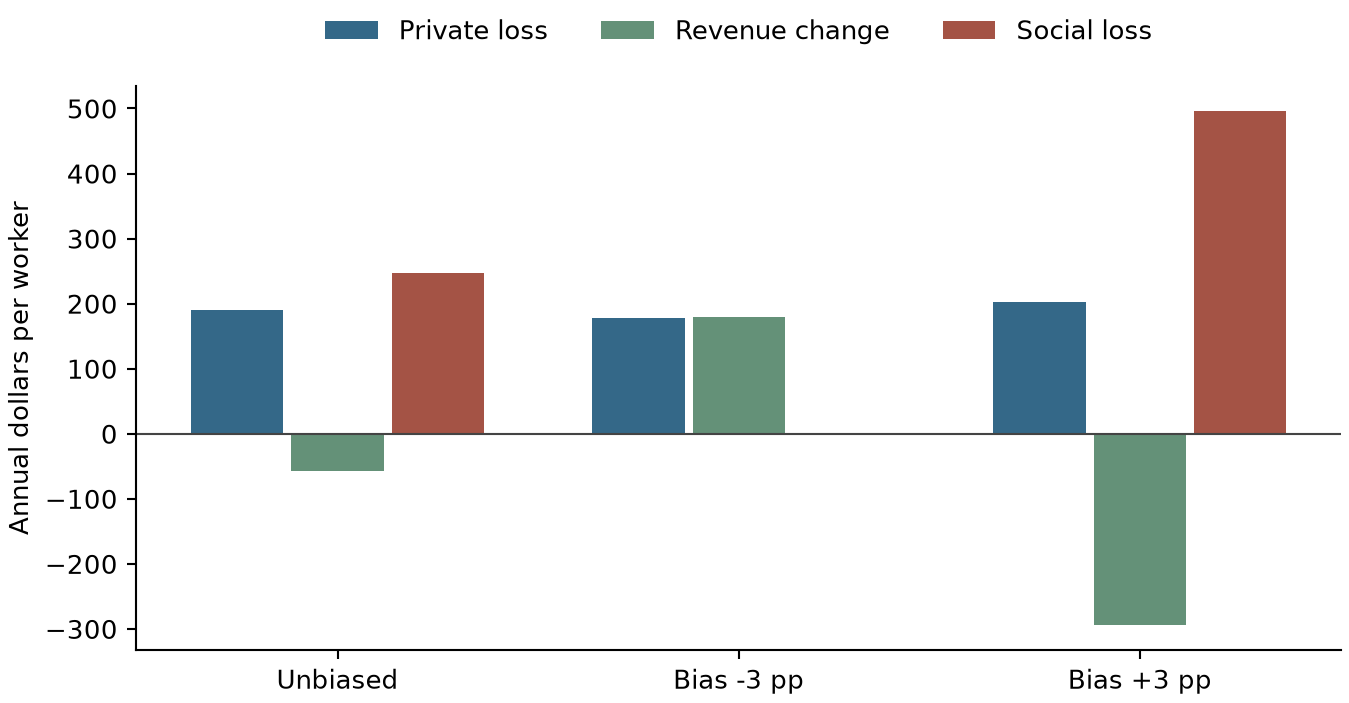
\includegraphics[width=1\linewidth,height=\textheight,keepaspectratio]{generated/welfare.png}

}

\caption{\label{fig-welfare}Private losses, revenue changes, and social
losses at the same latent RMSE. The common true tax rate is 30\%; all
values are illustrative annual dollars.}

\end{figure}%

\subsection{Optimal taxation is conditional on bias and social
weights}\label{optimal-taxation-is-conditional-on-bias-and-social-weights}

Under inverse-wage welfare weights, the informed optimum is 44.53\%. The
unbiased-error optimum is 42.93\%, while the scenario with a three-point
downward bias and the same latent RMSE has an optimum of 45.63\%. A
common RMSE therefore does not imply a common direction of the tax
response. Equal social dollar weights yield different optima because the
redistribution motive changes.

\begin{longtable}[]{@{}lrr@{}}
\caption{Best linear tax rates on the specified grid over 0\% to 80\%.
Zero is a search boundary, not a claim about an unconstrained
optimum.}\label{tbl-planner}\tabularnewline
\toprule\noalign{}
Scenario & Equal weights (\%) & Inverse-wage weights (\%) \\
\midrule\noalign{}
\endfirsthead
\toprule\noalign{}
Scenario & Equal weights (\%) & Inverse-wage weights (\%) \\
\midrule\noalign{}
\endhead
\bottomrule\noalign{}
\endlastfoot
No error & 0.00 & 44.53 \\
Unbiased & 0.00 & 42.93 \\
Bias -3 pp & 0.00 & 45.63 \\
Bias -6 pp & 0.00 & 48.50 \\
Bias +3 pp & 0.00 & 40.48 \\
Certain -1 pp & 0.95 & 45.38 \\
\end{longtable}

The comparison holds preferences, wage distribution, fiscal closure, and
the bounds on perceived rates fixed. It does not identify how a real
information intervention changes beliefs. Nor does it prove that the
optimum is globally monotone in noise. At very large noise levels,
censoring itself changes how beliefs respond to the true rate.

\subsection{Approximation accuracy and
sensitivity}\label{approximation-accuracy-and-sensitivity}

The exact utility calculation remains finite at boundaries where the
interior approximation is unreliable or undefined.
Table~\ref{tbl-accuracy} compares it with the historical formula using
the latent second moment. The discrepancy can reflect both changed
realized moments after censoring and failure of the local expansion.
Replacing the latent second moment with the realized one addresses the
former but does not make large behavioral errors local.

\begin{longtable}[]{@{}
  >{\raggedright\arraybackslash}p{(\linewidth - 6\tabcolsep) * \real{0.2000}}
  >{\raggedleft\arraybackslash}p{(\linewidth - 6\tabcolsep) * \real{0.2667}}
  >{\raggedleft\arraybackslash}p{(\linewidth - 6\tabcolsep) * \real{0.2667}}
  >{\raggedleft\arraybackslash}p{(\linewidth - 6\tabcolsep) * \real{0.2667}}@{}}
\caption{Approximation diagnostic in dollars, with informed earnings
normalized to \$55,000 separately at each true rate. The approximation
uses the latent second moment; the exact model censors perceived
rates.}\label{tbl-accuracy}\tabularnewline
\toprule\noalign{}
\begin{minipage}[b]{\linewidth}\raggedright
True rate (\%)
\end{minipage} & \begin{minipage}[b]{\linewidth}\raggedleft
Exact private loss
\end{minipage} & \begin{minipage}[b]{\linewidth}\raggedleft
Latent approximation
\end{minipage} & \begin{minipage}[b]{\linewidth}\raggedleft
Approx./exact
\end{minipage} \\
\midrule\noalign{}
\endfirsthead
\toprule\noalign{}
\begin{minipage}[b]{\linewidth}\raggedright
True rate (\%)
\end{minipage} & \begin{minipage}[b]{\linewidth}\raggedleft
Exact private loss
\end{minipage} & \begin{minipage}[b]{\linewidth}\raggedleft
Latent approximation
\end{minipage} & \begin{minipage}[b]{\linewidth}\raggedleft
Approx./exact
\end{minipage} \\
\midrule\noalign{}
\endhead
\bottomrule\noalign{}
\endlastfoot
0 & 71.90 & 130.68 & 1.82 \\
30 & 190.11 & 186.69 & 0.98 \\
80 & 962.90 & 653.40 & 0.68 \\
95 & 1,361.14 & 2,613.60 & 1.92 \\
99 & 1,561.56 & 13,068.00 & 8.37 \\
\end{longtable}

\begin{figure}

\centering{

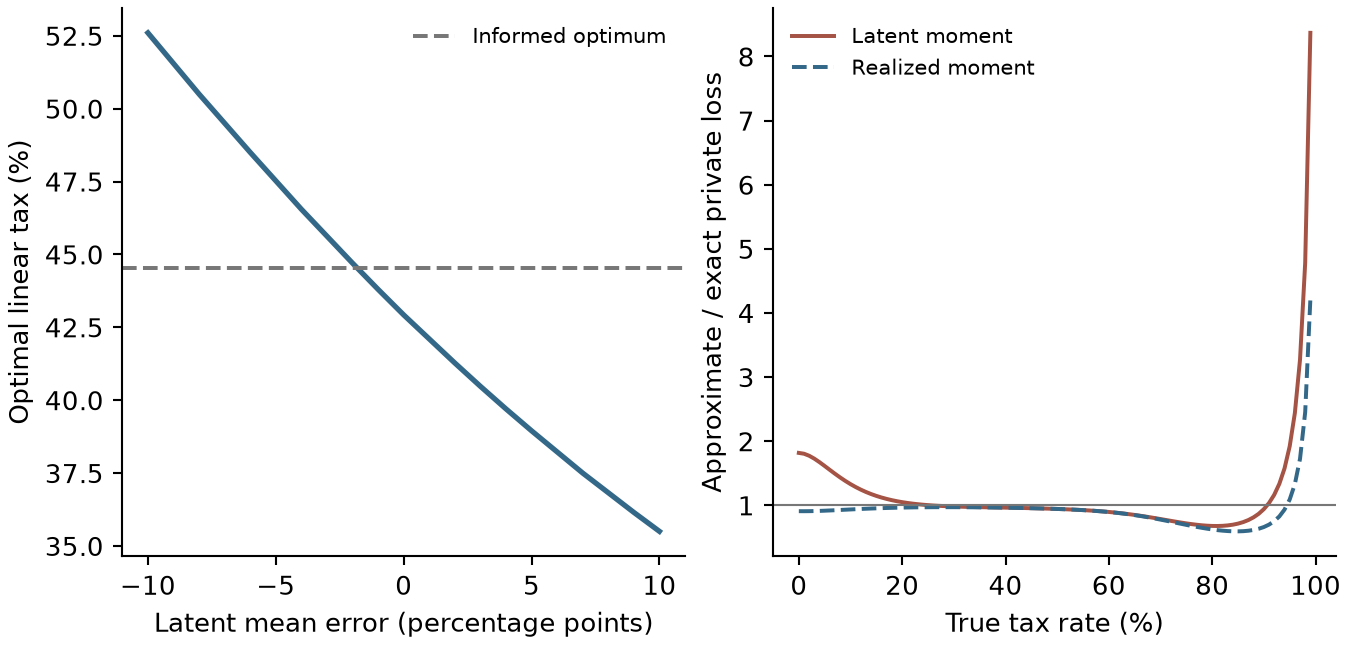
\includegraphics[width=1\linewidth,height=\textheight,keepaspectratio]{generated/robustness.png}

}

\caption{\label{fig-robustness}Left: the inverse-wage-weighted optimum
as bias changes while latent RMSE remains 12 points; the dashed line is
the informed optimum. Right: approximation error across true rates,
comparing latent and realized second moments. Informed earnings in the
right panel are separately normalized at each rate.}

\end{figure}%

\begin{longtable}[]{@{}lrrr@{}}
\caption{Illustrative social losses per worker in dollars under
mean-zero latent errors and equal valuation of rebated revenue. These
are scenario variations, not confidence
bounds.}\label{tbl-sensitivity}\tabularnewline
\toprule\noalign{}
Elasticity & SD 8 pp & SD 12 pp & SD 15 pp \\
\midrule\noalign{}
\endfirsthead
\toprule\noalign{}
Elasticity & SD 8 pp & SD 12 pp & SD 15 pp \\
\midrule\noalign{}
\endhead
\bottomrule\noalign{}
\endlastfoot
0.25 & 84.23 & 193.03 & 307.53 \\
0.33 & 108.10 & 247.09 & 392.37 \\
0.50 & 153.95 & 350.08 & 552.43 \\
\end{longtable}

The sensitivity table varies assumed elasticities and mean-zero error
dispersions. It describes the model across those inputs. It is not an
uncertainty interval around an empirically identified national estimate.

\section{Nonlinear budgets and actual household
outcomes}\label{nonlinear-budgets-and-actual-household-outcomes}

\subsection{Explicit nonlinear
schedules}\label{explicit-nonlinear-schedules}

A local MTR cannot describe a worker's alternatives across a bracket
boundary or a benefit cliff. The nonlinear implementation therefore
accepts a net-income function \(b(y)\) over an explicit earnings domain.
The worker maximizes
\(b(y)-\psi(y/w)^{1+1/\varepsilon}/(1+1/\varepsilon)\). On a known
affine segment, utility is strictly concave, so candidate maxima are its
stationary point and feasible endpoints. Evaluating candidates across
every segment finds the global maximum when it exists.

The schedule explicitly assigns each discontinuity's threshold to one
side. If a benefit disappears at a threshold and utility approaches a
superior value from below without attaining it, the continuous choice
problem can have a supremum but no maximizer. The solver reports this
case. It does not move the threshold or substitute an arbitrary epsilon.
A finite earnings grid is an alternative economic choice set with an
attained optimum.

Earnings subsidies, negative net-income slopes, and discontinuous
transfers are permitted. None are transformed into a tax rate capped at
99\%. The exact nonlinear accounting compares an informed choice with
the choice under a separate perceived budget, then evaluates both on the
true budget. Private regret is nonnegative on the common feasible choice
set. The change in \(y-b(y)\) supplies the net-revenue term only to the
extent that the budget measures all relevant taxes and transfers. The
government's complete fiscal cost can differ when the budget omits
benefits, externalities, or costs whose valuation differs from
consumption.

The numerical examples use a progressive schedule with net-income slopes
0.9 below \$30,000 and 0.65 above, a subsidy schedule with slopes 1.2
below \$15,000 and 0.7 above, and an \$8,000 benefit paid through
\$45,000 earnings that disappears above that point. The progressive and
subsidy budgets are continuous; the cliff assigns the threshold to the
benefit-receiving segment. Perceived net-income slopes are constant at
0.75, 0.8, and 0.7 respectively. Each example uses the illustrative
worker's preferences and a common feasible earnings range from zero to
\$100,000. All amounts are assumed.

\begin{longtable}[]{@{}lrrr@{}}
\caption{Synthetic nonlinear examples, dollars. True and perceived
budgets and exact choices are stored in the results; these are not
statutory schedules.}\label{tbl-nonlinear}\tabularnewline
\toprule\noalign{}
True budget & Private loss & Revenue change & Social loss \\
\midrule\noalign{}
\endfirsthead
\toprule\noalign{}
True budget & Private loss & Revenue change & Social loss \\
\midrule\noalign{}
\endhead
\bottomrule\noalign{}
\endlastfoot
Progressive & 127.69 & 908.37 & -780.67 \\
Earnings subsidy & 122.04 & 743.34 & -621.29 \\
Benefit cliff & 6,297.81 & 11,000.00 & -4,702.19 \\
\end{longtable}

\subsection{PolicyEngine household
grid}\label{policyengine-household-grid}

A separate adapter executes the pinned PolicyEngine household model
(PolicyEngine 2026) on an explicit earnings grid. The wrapper version is
5.3.0, with country model 1.764.6 and core 3.30.1. The stored fixture
records a single 40-year-old adult in Texas, filing singly, for 2024. It
contains 401 outcomes from zero to \$100,000 earnings and records the
wrapper/model versions, certified-bundle manifest, household inputs, tax
settings, grid resolution, and content hashes.

The outcome measure is PolicyEngine's household net income with health
benefits excluded. It includes some noncash benefits, so it is not
described as cash income or a complete fiscal account. The adapter
returns the observed grid without interpolation. The optimizer is exact
over those supplied choices; it cannot certify unseen cliff locations or
an error bound for the unknown continuous schedule between them.
Re-running a finer nested grid checks sensitivity to the finite choice
set, not statutory completeness.

\begin{longtable}[]{@{}lr@{}}
\caption{Selected actual PolicyEngine outcomes for the specified 2024
Texas household, in dollars. Health benefits are excluded; some other
noncash benefits are included.}\label{tbl-household}\tabularnewline
\toprule\noalign{}
Earnings & Household net income \\
\midrule\noalign{}
\endfirsthead
\toprule\noalign{}
Earnings & Household net income \\
\midrule\noalign{}
\endhead
\bottomrule\noalign{}
\endlastfoot
0.00 & 3,495.00 \\
25,000.00 & 22,047.50 \\
50,000.00 & 42,159.00 \\
100,000.00 & 78,509.00 \\
\end{longtable}

This fixture validates a real model connection and a transparent path to
household-level budget analysis. It is not used to estimate national
misperception losses. Such an estimate would additionally require
credible household-specific beliefs, labor preferences, feasible work
choices, treatment of other household members, fiscal valuations, and a
provenance-known population dataset. The former population calculation
that clipped MTRs and loaded year-only caches is retired explicitly.

\subsection{Preferences, learning, and information
provision}\label{preferences-learning-and-information-provision}

The retained Cobb-Douglas benchmark gives tax-invariant hours without
nonlabor income because income and substitution effects cancel. A
positive compensated elasticity alone does not rule out that
cancellation. The quasilinear model is not a special case of the
displayed homogeneous CES family in earlier drafts, and this note makes
no claim that its estimates bound welfare effects under other
preferences.

Dynamic learning, information-acquisition costs, participation, and job
constraints are omitted. Correcting a worker's beliefs improves that
worker's objective under a fixed budget and transfer, but may change tax
revenue and others' transfers. Ranking information interventions
requires their costs, their effects on behaviorally relevant beliefs,
and the chosen social objective. This model does not establish that
simplification dominates rate changes.

\section{Conclusion}\label{conclusion}

Tax misperception creates a private optimization loss in this model, but
its social effect depends on changes in revenue and the use of public
funds. The exact accounting identity makes that distinction visible.
Bias and dispersion have different fiscal implications, even when the
latent RMSE is the same. The illustrative planner results consequently
change direction when systematic underestimation replaces part of the
unbiased noise.

The contribution is a reproducible framework and a set of conditional
numerical checks. The earlier national dollar estimates are withdrawn:
neither the assumed error distribution nor the clipped-MTR aggregation
established them. Empirical work should first identify the
decision-relevant error distribution and its relationship to income and
tax provisions. Household budget analysis can then retain
nonlinearities, state its feasible work choices, and record the
tax-model and data provenance needed for replication.

The calibration adapter also reproduces selected Rees-Jones/Taubinsky
benchmarks from native replication data and bounds signed errors implied
by retained experimental choices. Tests verify the raw-choice mapping,
selection, provenance and moment inequalities. These observed interval
results complement the welfare framework while leaving response noise,
stable latent beliefs and population and tax-component coverage
unresolved. The illustrative welfare inputs remain separate from this
scoped empirical evidence.

\section{Derivation and numerical
checks}\label{derivation-and-numerical-checks}

\subsection{Private-regret expansion}\label{private-regret-expansion}

Let \(q=1-\tau>0\). At the informed interior optimum, \(u_h=0\) and
\(u_{hh}=-wq/(\varepsilon h^0)\). The response to a small realized error
is

\[\Delta h=-\frac{\varepsilon h^0}{q}e+\frac{\varepsilon(\varepsilon-1)h^0}{2q^2}e^2+O(e^3).\]

Substitution into the second-order utility expansion gives

\[P\approx\frac{1}{2}|u_{hh}|E[(\Delta h)^2]=\frac{\varepsilon y^0}{2q}E[e^2].\]

The same hours expansion gives \(\Delta R=\tau wE[\Delta h]\). The
social-loss identity follows by adding the expected change in the
balanced-budget transfer to private utility, with the specified social
dollar weights. It does not require a Taylor approximation.

\subsection{Expectation and
optimization}\label{expectation-and-optimization}

The primary linear calculation integrates the normal density
deterministically, including probability masses at censoring bounds.
Integration intervals are split at the zero-hours corner. A change of
variables resolves the fractional-power labor-supply behavior there.
Uncensored tails beyond 12 standard deviations are omitted and
probabilities normalized; this probability approximation is negligible
for the reported parameter range. Numerical convergence is checked by
increasing quadrature order, and independent Monte Carlo checks evaluate
utility and balanced transfers directly.

For the planner, common preferences and a belief distribution
independent of wages allow wage moments and belief moments to be
evaluated separately. Expected labor disutility uses the expected power
of hours, not the power of expected hours. The default tax search spans
0 to 0.8 with 81 grid points, followed by another 81-point grid around
the coarse maximum. The final grid spacing and boundary status are
stored.

Tests cover no-error identities, the small-error limit, signed-bias
fiscal effects, equal and inverse-wage objectives, negative true rates
with compatible belief bounds, corners at and above a 100\% tax,
censored moments, explicit nonlinear thresholds, subsidies, and discrete
grid optimization. A deterministic one-point underestimate is checked
against direct realized utility. Zero private regret and zero fiscal
change are required in an informed comparison whenever the chosen belief
bounds contain the true rate.

\subsection{Replication and scope
controls}\label{replication-and-scope-controls}

The default pipeline generates only synthetic scenarios. Source
fingerprints and explicit assumptions accompany the versioned results.
Quarto reads generated tables and variables; a check command compares
recomputed numbers and paper artifacts to their stored versions. A
separately enabled PolicyEngine check runs an actual household model and
verifies the finite-grid interpretation. Stored household artifacts
carry their complete request and model provenance. Unknown legacy cache
provenance is rejected.

The model has no calibrated national sample, no estimated intervention
effect on beliefs, and no general-equilibrium wage response. Social
welfare calculations use a stated rebate rule and social dollar weights.
These limits are part of the estimand rather than adjustments that can
be inferred after computing a population total.

\section{Appendix: Study 1 calibration evidence}\label{sec-study1-audit}

Study 1 of Rees-Jones and Taubinsky (2020) supports reproducible
\textbf{finite-design forecast projections}, with substantial selection
and measurement limitations. It does not separately identify stable
individual marginal-tax beliefs or their latent variance. This appendix
integrates a separately audited calculation; the original authors did
not report the projection-error and sensitivity tables below. The pooled
Table 1 benchmarks and all Study 2 findings above are unchanged.

\subsection{Retained sample, processing and true-tax
support}\label{retained-sample-processing-and-true-tax-support}

The native archive contains 74,128 forecasts from 4,633 people. Applying
\texttt{attention==0} retains 67,152 forecasts from 4,197 people. The
article's earlier 195 exclusions and original rolling winsorization
cannot be rerun from these retained files. The 58,758 rows in
\texttt{individualestimates.dta} reuse the same random-income answers:
all 31 audited numeric fields match, so this file supplies no
independent remeasurement. The main outcome \texttt{taxguessmain} equals
\texttt{tgw1}. Relative to retained pre-winsorization
\texttt{taxguessds}, 958 differences arise only from float32 storage
conversion; 543 exceed that conversion, affecting 289 people. These
differences do not isolate response noise. For the full random-income
design, observed error SD is 16.89 pp with the main outcome, 43.33 pp
before winsorization, and 13.45 pp with the retained \texttt{tgw5}
alternative.

The native local flag is
\texttt{(qnum\textless{}=2)\ or\ (bracket==ownbracket)} and includes 89
forecasts outside the respondent's own nominal bracket. Even bracket
matching does not establish a locally affine true tax function. Of 3,471
respondents with at least three distinct own-bracket incomes, 13 fail an
\textbf{observed affine screen}: maximum absolute residual from an OLS
line through stored true liabilities must be at most \$0.05. Their 30
affected forecasts carry positive stored exemption phaseout. The maximum
departure from the nominal own-rate line is \$2,189.88. A separate
stored-field calculation reconciles that departure to the
exemption-phaseout tax amount within \$0.0050963. This checks archived
arithmetic; the missing liability-generation code prevents certification
of the complete legal schedule. Passing at observed points does not
establish affinity between them, and a perfect two-point fit supplies no
such test.

For each respondent, regress the forecast on income with an intercept
and subtract the slope of stored true tax on the \textbf{same incomes}.
This signed projection error has units of tax dollars per income dollar;
multiply by 100 for percentage points. It is not automatically a
point-MTR error. Unlike the pooled tax-on-tax coefficient, which weights
people by within-person true-tax variation, the descriptive moments
below give each person equal mass and use variance denominator \(N\).

\begin{longtable}[]{@{}lrrr@{}}
\caption{Study 1 finite-design signed slope errors using processed
forecasts. Counts 3+/4+ mean distinct observed incomes; span cutoffs are
dollars. The observed affine screen requires at least three incomes and
maximum stored-tax OLS residual at most \$0.05. Equal respondent mass;
SD denominator N. No slope clipping or latent-noise
correction.}\label{tbl-study1-selection}\tabularnewline
\toprule\noalign{}
Income design & N & Median span (\$) & Error SD (pp) \\
\midrule\noalign{}
\endfirsthead
\toprule\noalign{}
Income design & N & Median span (\$) & Error SD (pp) \\
\midrule\noalign{}
\endhead
\bottomrule\noalign{}
\endlastfoot
Own-income pair & 4,197 & 502 & 83,579.42 \\
Native local & 4,197 & 17,246 & 6,373.28 \\
Own bracket: 3+, affine & 3,458 & 22,721 & 208.96 \\
Own bracket: 4+, affine, span 5k+ & 2,470 & 31,516 & 45.08 \\
Own bracket: 4+, affine, span 10k+ & 2,279 & 33,465 & 32.14 \\
All 14 random draws & 4,197 & 424,167 & 16.89 \\
\end{longtable}

The extreme short-span SDs are untrimmed calculations, not unit
mistakes. Liability winsorization does not cap slopes divided by small
income differences. Requiring four distinct own-bracket incomes, at
least \$5,000 support and the observed affine screen leaves 2,470
people. Their mean signed error is +0.70 pp, but this precision screen
raises median own income from \$45,000 to \$62,237. The sample and
estimand therefore change with the screen. The smaller full-range SD
also does not validate local beliefs: every respondent's full-range
stored true-tax values fail the affine screen.

\subsection{Compatibility with an assumed answer-error
cap}\label{compatibility-with-an-assumed-answer-error-cap}

For an assumed dollar cap \(a\), ask whether \textbf{some} intercept
\(\alpha\) and unrestricted slope \(\beta\) satisfy

\[|y_{ij}-\alpha-\beta x_{ij}|\leq a\quad\text{for every retained answer }j.\]

For every pair with \(x_j>x_k\), intersect the intervals
\([(y_j-y_k-2a)/(x_j-x_k),(y_j-y_k+2a)/(x_j-x_k)]\); equal-income pairs
additionally require \(|y_j-y_k|\leq2a\). This is necessary and
sufficient because the implied intercept intervals have a common
intersection exactly when they overlap pairwise. Writing the
intersection bounds as \(L,U\), the implementation closes a reversed
endpoint gap only when \(L-U\leq10^{-12}\max(1,|L|,|U|)\), in
slope-fraction units; this is numerical tolerance, not a larger
dollar-error cap. The minimum feasible cap is
\(\tfrac12\min_\beta[\max_j(y_j-\beta x_j)-\min_j(y_j-\beta x_j)]\).

\begin{longtable}[]{@{}lrrr@{}}
\caption{Compatibility with some affine forecast function and an assumed
uniform dollar-error cap in the 2,470-person screened sample. Width is
the feasible slope-set width among compatible respondents only; shares
are not identified belief
types.}\label{tbl-study1-affine}\tabularnewline
\toprule\noalign{}
Cap per answer (\$) & Compatible / N & Share (\%) & Median width (pp) \\
\midrule\noalign{}
\endfirsthead
\toprule\noalign{}
Cap per answer (\$) & Compatible / N & Share (\%) & Median width (pp) \\
\midrule\noalign{}
\endhead
\bottomrule\noalign{}
\endlastfoot
50 & 424 / 2,470 & 17.2 & 0.76 \\
100 & 555 / 2,470 & 22.5 & 1.51 \\
500 & 1,084 / 2,470 & 43.9 & 6.90 \\
1,000 & 1,411 / 2,470 & 57.1 & 13.23 \\
5,000 & 2,132 / 2,470 & 86.3 & 61.83 \\
\end{longtable}

The median minimum cap is \$693.29. Failure rejects the \textbf{joint
affine-forecast model and assumed cap}; it does not identify curved
beliefs, response mistakes, stable belief types or irrationality.
Passing does not establish temporal stability. In particular, the
555/2,470 result at a \$100 cap is not a type share. The experiment's
\$100 accuracy window for earning a \$1 bonus does not bound answer
errors. Retaining only compatible respondents would add outcome-based
selection.

Without requiring affine beliefs, a cap \(|u_{ij}|\leq a\) bounds the
difference between observed and latent \textbf{projected} slopes by
\(a\sum_j|x_{ij}-\bar x_i|/S_{xx,i}\). At an assumed \$100 cap, its
median radius is 39.84 pp for the own-income pair versus 0.73 pp in the
screened sample. These deterministic sensitivities permit biased,
correlated noise; the cap is not estimated. Without a noise restriction,
no finite latent upper bound follows.

\subsection{Within-survey covariance and unidentified latent
variance}\label{within-survey-covariance-and-unidentified-latent-variance}

The archive contains only one incidental exact-income repeat, with a
\$401 forecast discrepancy, and no independent waves. Instead, sorting
each person's draws by \texttt{(ran,qnum)} and alternating them creates
two disjoint income designs. Each half must contain at least two
distinct incomes; \texttt{qnum} denotes sampling slots, not a verified
presentation order. Among own-bracket respondents passing the observed
affine screen, requiring each half to span at least \$5,000 leaves 1,986
people. The covariance of their signed error projections is 309.05
pp\(^2\), with delete-one-person jackknife SE 152.55 pp\(^2\) and
correlation approximately 0.1002613. Covariance uses denominator
\(N-1\); both it and its SE multiply by 10,000 when converting squared
fractions to pp\(^2\). The jackknife describes sampling variation under
independent respondents, not a measurement-error correction.

Under \(s_A=\theta+u_A\), \(s_B=\theta+u_B\), covariance equals
\(\operatorname{Var}(\theta)\) only if both errors are orthogonal to the
\textbf{same} target and to each other. Curved beliefs and different
income supports may violate the common-target assumption. Homoskedastic
iid residual SEs assume a correct line and independent answer errors;
HC3 allows heteroskedasticity but does not remove shared response
errors. Splitting one survey is not test-retest measurement.

Even granting a common target and orthogonality to it, error correlation
\(\rho\) changes the variance decomposition:

\[C=V+\rho\sqrt{(V_A-V)(V_B-V)},\qquad 0\leq V\leq\min(V_A,V_B).\]

Here the sample moments in squared fractions are \(V_A\) = 0.2824215363,
\(V_B\) = 0.3364288928 and \(C\) = 0.0309050061.

\begin{longtable}[]{@{}lr@{}}
\caption{Conditional second-moment decompositions for N=1,986. Errors
are assumed orthogonal to the same latent target. The last row uses the
observed correlation, displayed rounded; the exact zero-variance
identity does not hold at a literal correlation of 0.100000. These are
sensitivities, not estimates of error correlation or latent
variance.}\label{tbl-study1-covariance}\tabularnewline
\toprule\noalign{}
Assumed error correlation & Implied common-target SD (pp) \\
\midrule\noalign{}
\endfirsthead
\toprule\noalign{}
Assumed error correlation & Implied common-target SD (pp) \\
\midrule\noalign{}
\endhead
\bottomrule\noalign{}
\endlastfoot
0.0000000 & 17.58 \\
0.0501306 & 12.76 \\
0.1002613 & 0.00 \\
\end{longtable}

At \(\rho=0\), \(V=C\); at \(\rho=C/\sqrt{V_AV_B}\), \(V=0\) reproduces
the same second moments. This admissible decomposition neither estimates
actual noise correlation nor proves zero stable heterogeneity. The
archive supplies no restriction that selects one decomposition.

The hypothetical 2014 federal salary-tax filer, standard deduction and
absence of additional credits/deductions also limit coverage.
Recruitment approximating some census demographics does not establish
representative latent beliefs; state taxes, payroll taxes, benefits and
behavioral transport remain unmeasured. None of these projection SDs,
compatibility shares or conditional decompositions replaces the model's
\textbf{illustrative latent RMSE of 0.12} or identifies a national
welfare calibration.

The repository's \texttt{calibration/study1/README.md} documents
reproduction from the checksum-pinned archive. Its manifest preserves
the minimal aggregate inputs and audit code at reviewed commit
\texttt{a5191ea}, with the later report precision clarification recorded
separately. The normal pipeline generates the appendix tables and inline
values from that evidence cache. Raw microdata, original source code and
source PDFs are not redistributed; their licensing restrictions remain
unchanged.

\newpage{}

\section*{References}\label{references}
\addcontentsline{toc}{section}{References}

\protect\phantomsection\label{refs}
\begin{CSLReferences}{1}{1}
\bibitem[\citeproctext]{ref-chetty2012bounds}
Chetty, Raj. 2012. {``Bounds on Elasticities with Optimization
Frictions: A Synthesis of Micro and Macro Evidence on Labor Supply.''}
\emph{Econometrica} 80 (3): 969--1018.
\url{https://doi.org/10.3982/ECTA9043}.

\bibitem[\citeproctext]{ref-policyengine2026}
PolicyEngine. 2026. \emph{PolicyEngine Python Interface}. Version 5.3.0.
\url{https://pypi.org/project/policyengine/5.3.0/}.

\bibitem[\citeproctext]{ref-rees2020schmeduling}
Rees-Jones, Alex, and Dmitry Taubinsky. 2020. {``Measuring
{`Schmeduling'}.''} \emph{Review of Economic Studies} 87 (5): 2399--438.
\url{https://doi.org/10.1093/restud/rdz045}.

\end{CSLReferences}




\end{document}
